\section{Smart meter context model}
\begin{figure}
  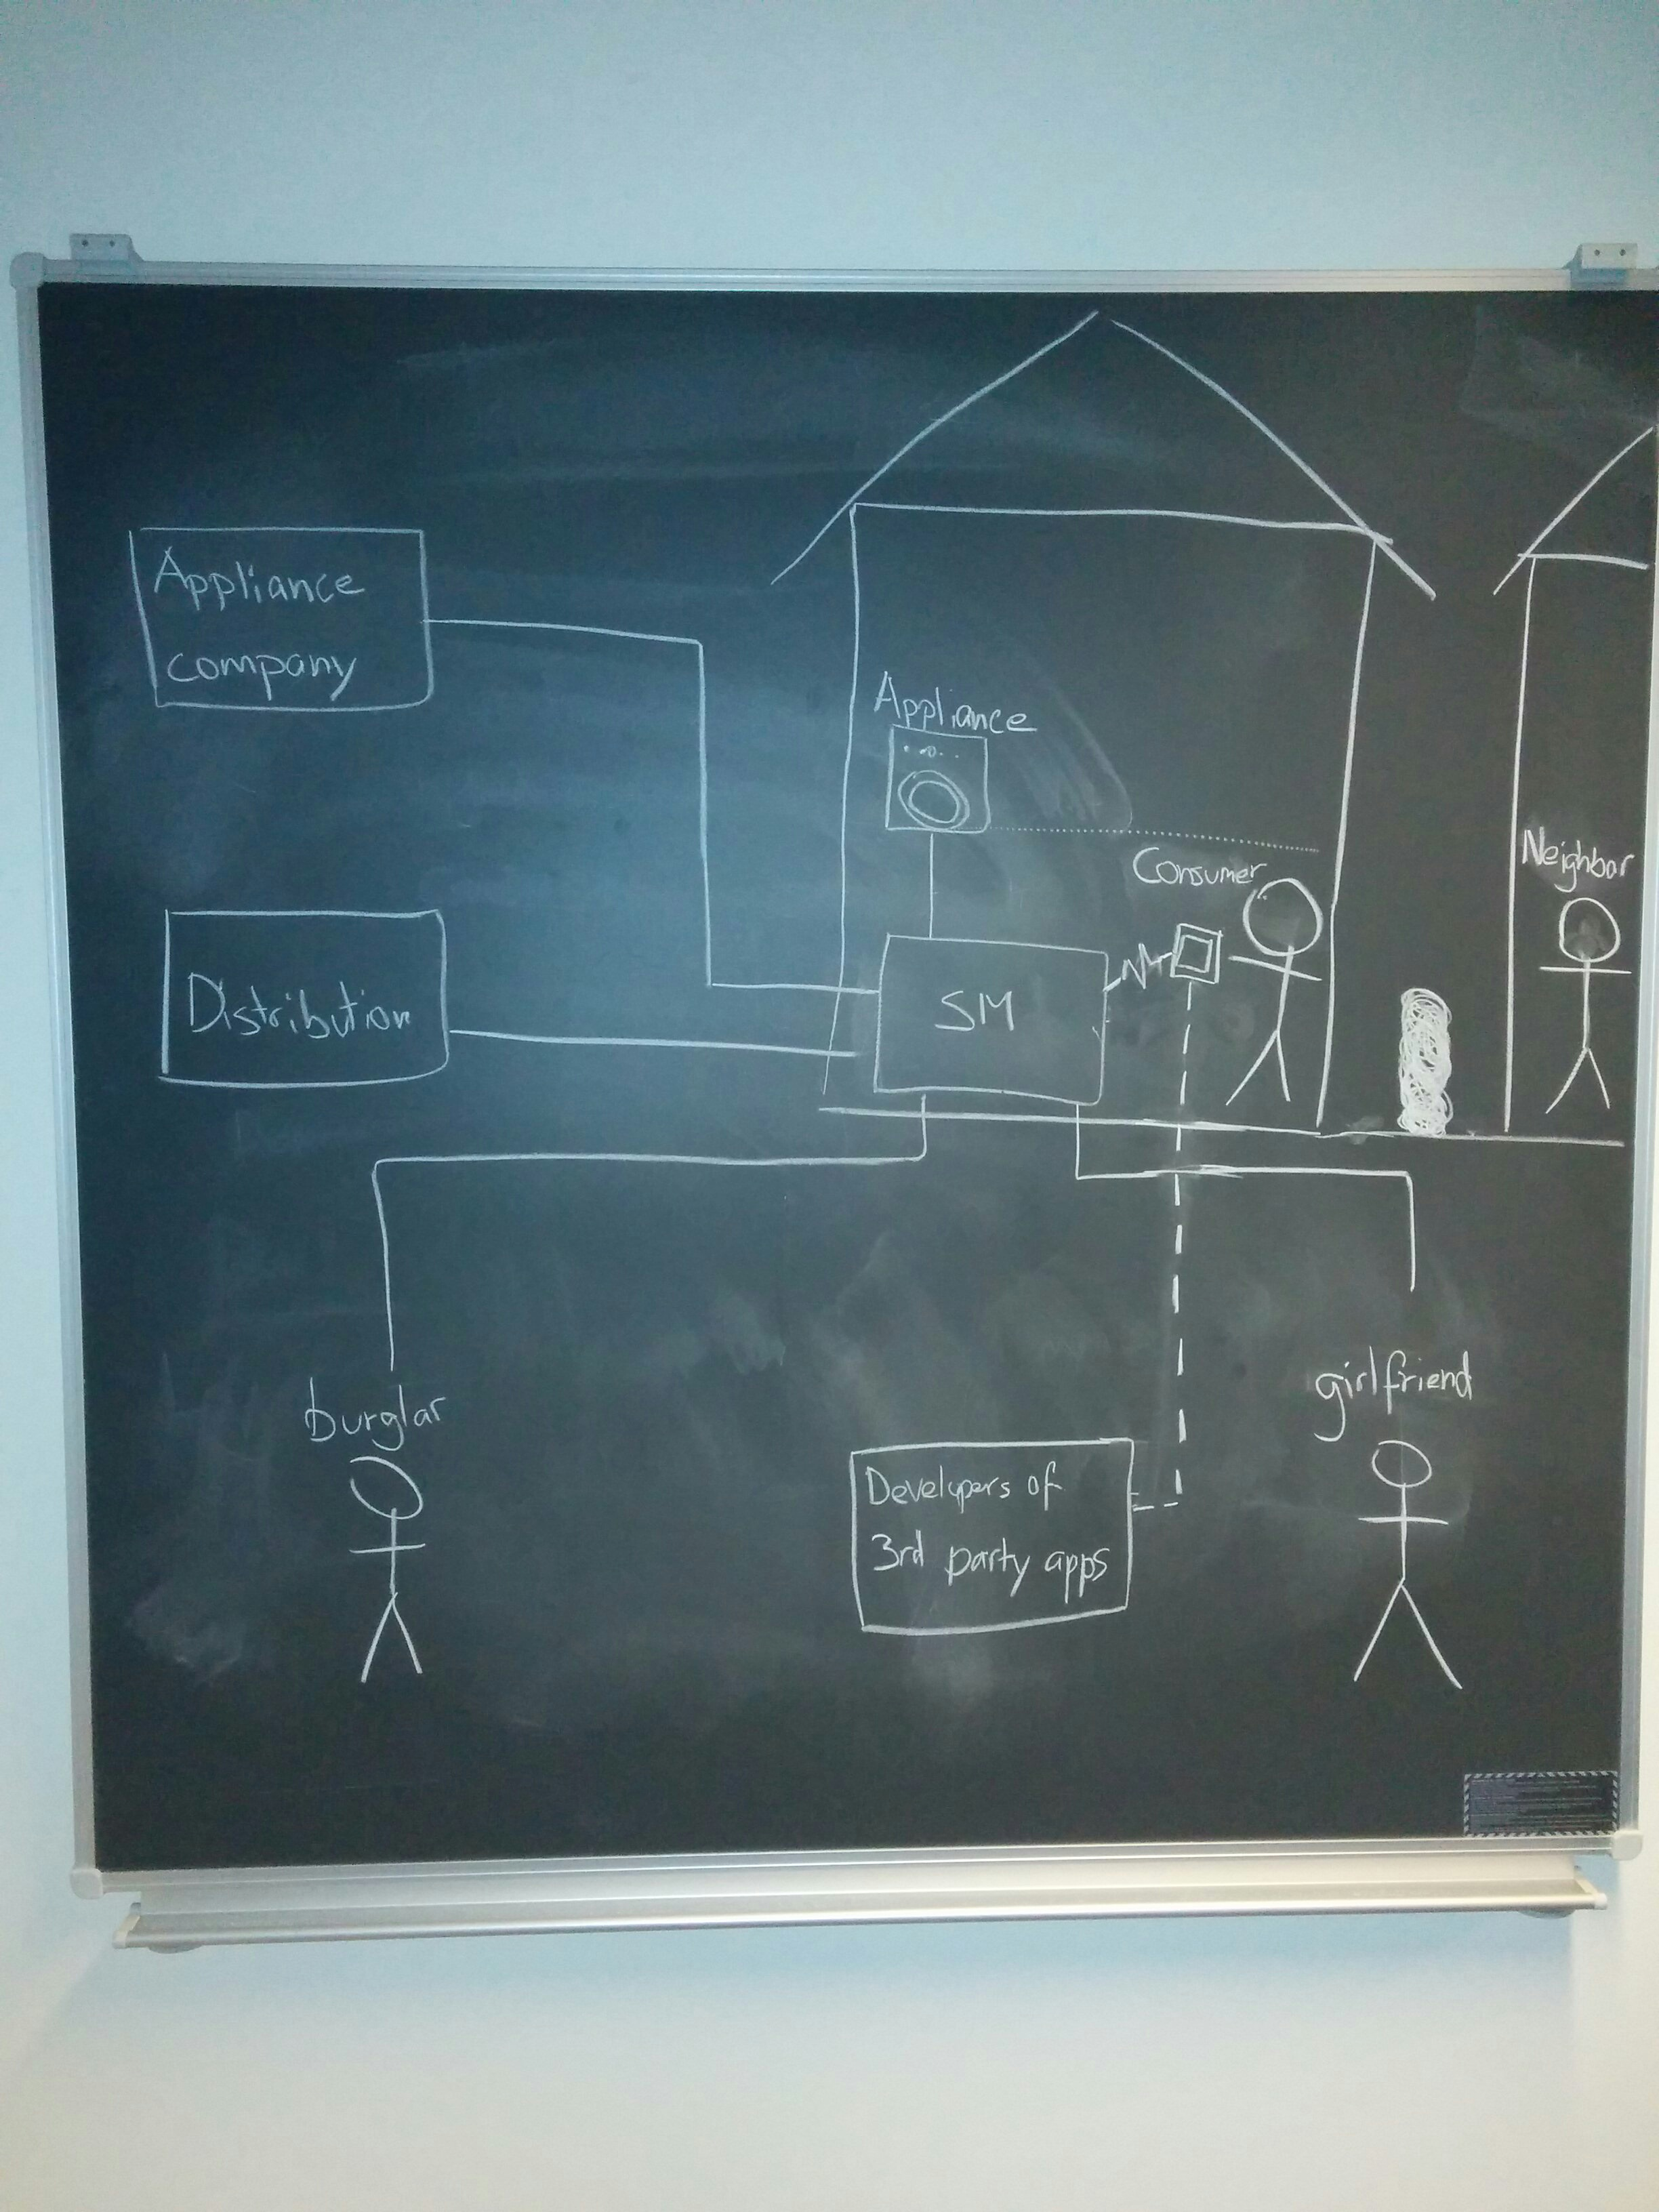
\includegraphics[width=\textwidth]{figures/situation.jpg}
  \caption{Smart meter context model.}
  \label{sm_model}
\end{figure}

\subsection{Actors}
List of actors in the model.
\begin{itemize}
\item Consumer - is the one that has the SM installed at their household.
\item Distribution - the provider of the electricity network and the SM, both hardware and software.
\item Developers of third party apps - the developer of apps that the consumer will use for seeing his electrical consumption. Can be both mobile, desktop and web applications
\item Appliance company - the provider of home appliances that can collaborate with the SM.
\item Burglar - wants to find out when the consumer is home in order to break in, what products the consumer own in order to assess him as a target
\item Girlfriend - wants to spy on the husband, take revenge on her ex-boyfriend.
\item Neighbour - wants to payback his annoying neighbour.
\end{itemize}

\subsection{Objects}\bruno{Better name!?}
\begin{itemize}
\item Smart meter(SM) - controls home appliances and also records consumption for each.
\item Appliance - has an option to be controlled from the smart meter. For instance a washing machine can be started and stopped when scheduled.
\end{itemize}

The smart meter is installed in the household of the consumer, in this case a house.
Home appliances are connected to the SM through their power cable, which provides electricty and information exchange.
The SM can be accessed through an API with different levels of rights, depending on the actor.
The consumer can access and manage his home appliances connected to the smart meter through some sort of program for instance an app, developed by a third party.
The girlfriend has access to the SM by having a password from the consumer or having her own account.
The distribution has the ability to update software, check the consumption and switch off the SM.
The home appliance company can update the firmware of their appliances through the SM.
The burglar and the Neighbour can try to access the SM through the API or physically at the household.
